\chapter{Overview of LPDDR4X}

\section{DRAM and LPDDR4X}
DRAM, or dynamic random access memory, is a type of volatile memory that is widely used in digital electronic systems. Volatile memory is a type of memory that loses its stored data when the power is turned off. DRAM operates by storing each data bit in a separate capacitor within a memory cell. The charge stored in each capacitor represents the binary value of the bit.

To maintain the data stored in the memory cells, a periodic refresh operation must be performed, hence the name “dynamic” memory. The refresh operation essentially rewrites the data in the memory cells to prevent the loss of data as the charge in the capacitor of a memory cell leaks out of the cell.

In DRAM, data is accessed randomly, as any memory location can be accessed directly without having to access the memory in a specific order, hence the term “random access” memory. This random access capability of DRAM provides faster access to data compared to other types of memory, such as magnetic disk drives.

DRAM technology is based on a capacitor-transistor (C-T) cell, which consists of an access transistor and a trench capacitor \cite{BORA}. The transistor allows current to go through and control the flow of charge to and from the capacitor. During a read operation, the charge stored in the capacitor is sensed and converted into a digital voltage signal, which represents the binary value of the data. During a write operation, the voltage signal is converted into a charge and stored in the capacitor.
DDR stands for double data rate and is an indication of the device sampling data and sending data twice per clock cycle. This is done by sampling the data on crossing points of a differential clock pair. Figure \ref{fig:dram-io} depicts the signals for double data sampling. 
A memory device is organized to maximize memory bandwidth and minimize the latency of operations. The organization of a DRAM module allows the designer of the memory controller to take advantage of parallel channels and structures to increase the data bandwidth. 

The device specification of each generation such as LPDDR4 (Low-power Double Data Rate) is defined by the JEDEC organization \cite{jedec}. Table \ref{tab:standards} shows multiple generations of the DDR standards up to DDR4 and the corresponding clock rate and transfer bandwidth \cite{patterson}. Amdahl's law suggests that the capacity of DRAM devices needs to grow linearly with the processor speeds; however, the performance and capacity of DRAM devices are growing at a much slower rate \cite{patterson}. 
\begin{table}[]
    \centering
    \begin{tabular}{c|c|c|c|c}
         Standard & Release Year & Capacity & I/O Clock Rate & MiB/s/DIMM \\
         \hline
         DDR1 & 2000 & 256 MB & 133 & 2128 \\
         DDR2 & 2004 & 1 GB & 266 & 4264 \\
         DDR3 & 2010 & 4 GB & 533 & 8528 \\
         DDR4 & 2016 & 8 GB & 1333 & 21300\\
    \end{tabular}
    \caption{DDR standards \cite{patterson}.}
    \label{tab:standards}
\end{table}
Functional description, detailed device operations, bus operations, cycle-accurate timings, and nominal conditions of operations are described in the 
specification for each generation. 
\section{DRAM Organization}

\begin{figure}[h]
    \centering
    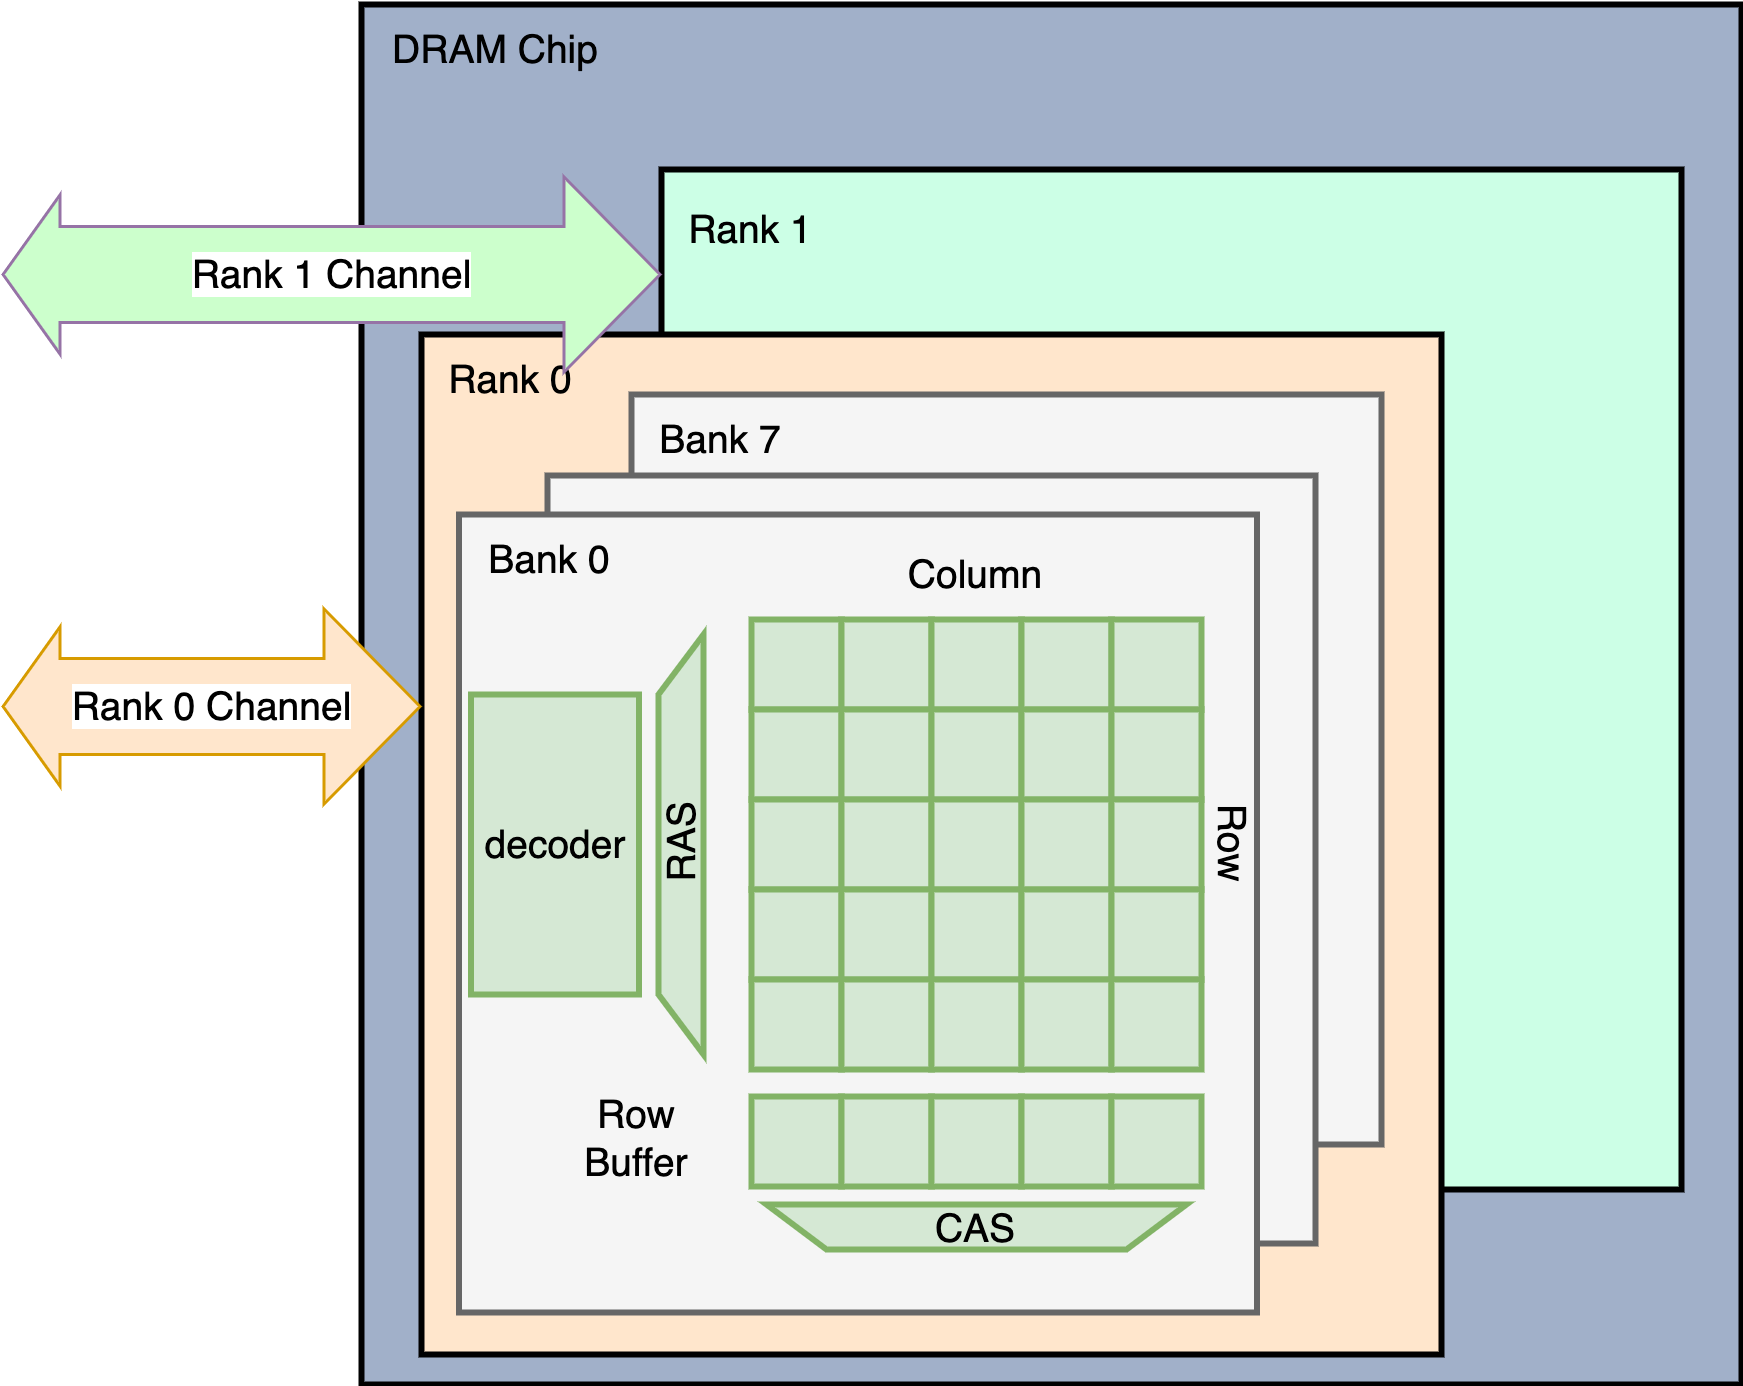
\includegraphics[scale=.14]{images/rank-bank.png}
    \caption{DRAM device organization.}
    \label{fig:rank-bank}
\end{figure}

DRAM devices are optimized to increase the bandwidth of the memory channels. The metric for such optimization is the activity of the DQ lanes between the DRAM and the controller. DQ is a bi-directional bus between the device and the memory controller. The organization and internals of the DRAM device dictate the complexity and responsibilities of a DRAM controller. As depicted in Figure \ref{fig:rank-bank}, a typical LPDDR4X device is organized into two physically separated ranks. Each rank of the device can be configured and connected to a separate channel. These two ranks can be active simultaneously and operate independently of each other. Each rank is organized into 8 banks of memory. The states of these banks impact the overall state of the memory device. Each bank is a two-dimensional memory array with column and row addresses. The memory array is structured as capacitor-based bit-cells with an access transistor for accessing the data stored in the capacitor. A row can store a large set of bytes and can extend to multiple system cache lines. A subset of the row is selected by multiplexers based on the column address. To perform a read transaction: the corresponding bank within the rank must be selected based on the address; the row for which the address maps to is selected, and the columns corresponding to the requested address are selected. Each operation must perform a sequence of specified commands to be issued to a bank for the purpose of reliably reading the data from the memory. The example read operation above would require activation of the row or row access (RAS), followed by a column access command (CAS), and finally by a pre-charge command (PRE). The timing and latencies between each step are specified by the JEDEC specification and the memory controller is responsible for obeying them. Overall, the memory controller is responsible for issuing the right sequence of commands at the right time to the device. Internally the memory controller must keep track of the state of the device at each cycle, allow the legal commands to be issued at any point, and force the right ordering of the commands. The timing requirements introduce the opportunity to optimize the memory controller to take full advantage of the possible bandwidth by allowing the architect to re-order requests, delay a pre-charge, or delay a refresh.
\section{DRAM Interface}
\begin{figure}
    \centering
    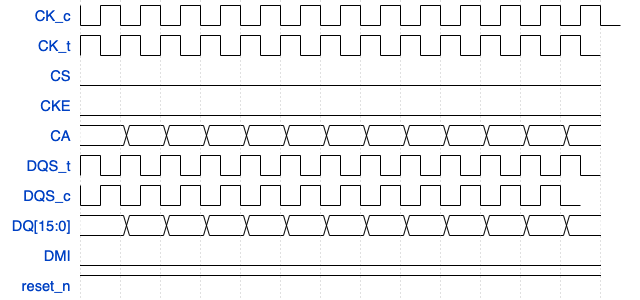
\includegraphics[scale=0.5]{images/signals.png}
    \caption{Waveform of device signals.}
    \label{fig:dram-io}
\end{figure}
\begin{figure}
    \centering
    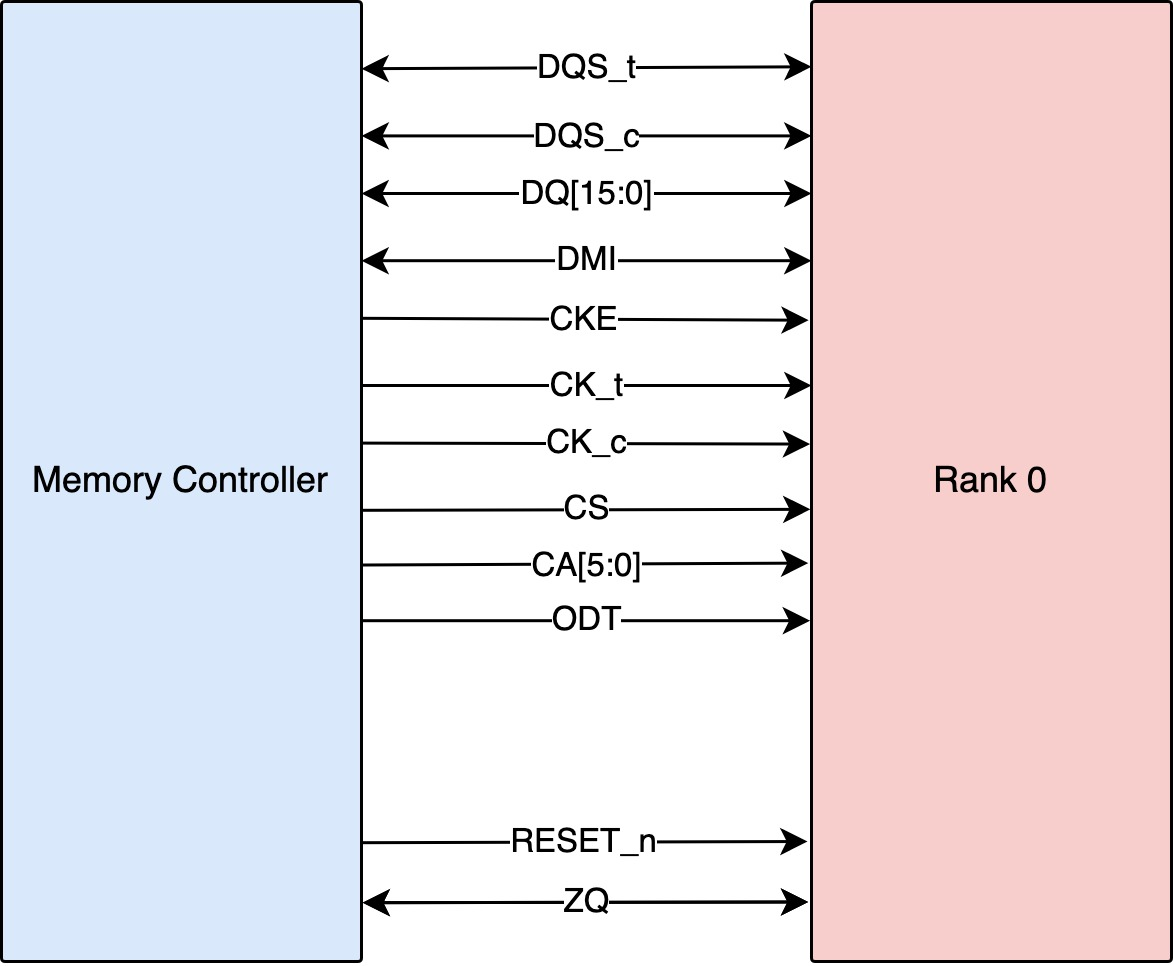
\includegraphics[scale=0.2]{images/signal-int.jpg}
    \caption{Signal interface for x16.}
    \label{fig:sig-int}
\end{figure}

The JEDEC specification determines the standard signals to be driven by the DDR controller and the DRAM device. An example of a signal waveform is shown in Figure \ref{fig:dram-io}. A description of each signal is shown based on the JEDEC specification in Table \ref{tab:signal-def}. Each LPDDR4X DRAM device is divided into two ranks which are connected in parallel to a dedicated channel. Signals such as CK\_t and CK\_c are shared among the two channels; however, the DQ bus, the CA bus, and the corresponding differential DQS clocks are separate between the two channels. 
\begin{table}[]
    \centering
    \begin{tabular}{c|c|c}
         Symbol & Type &  Description\\
         \hline
         CK\_t | CK\_c & Input & Clock: CK\_t and CK\_c are differential clock inputs\\
         CKE & Input & Clock Enable: Active high signal\\
         CS & Input & Chip Select \\
         CA[5:0] & Input & Command and Address Inputs\\
         ODT & Input & On-Die-Termination control\\
         DQ[15:0] & I/O & Bi-directional data input and output\\
         DQS\_t | DQS\_c & I/O & Data Strobe, Bi-directional differential clock signal\\
         DMI & I/O & Data Mask Inversion \\
         ZQ & Reference & Calibration Reference \\
         RESET\_n & Input & Active low reset signal
    \end{tabular}
    \caption{Signal Description for x16.}
    \label{tab:signal-def}
\end{table}
\newpage
\section{Prior Work}
Research on memory controllers in universities and among academics has a very short background. To our knowledge, many other research institutions either do not work in this area, or purchase vendor IP to integrate in their design. In the open-source community, LiteDRAM by EnjoyDigital \cite{enjoydigital} is an implementation of a DDR4 controller that can be mapped to FPGA systems. However, for the purposes of enabling more research work to be done in this area, an open-source controller is required.
\section{Project Goals}
The target for this project was to design an open-source LPDDR4X controller to be used as an IP in chip designs, and to be used to study a complete SoC. Interesting work such as studying DRAM targetted attacks, system-level analysis, and reordering of transactions will be possible using such IPs. The project will result in a generator in Chipyard \cite{chipyard}. Chipyard will provide an SoC designer with simple-to-use configuration-based knobs to include IPs such as an LPDDR4X controller in a design.